	\chapter{Machine Learning Pipeline and Hyperparameter Tuning}

	\resetquestioncounter{}
	\begin{qanda}
		\begin{question}
What is the difference between fit, fit\_transform, and transform?
		\end{question}

		\begin{answer}
The way we use fit and predict in regression, similarly for functions that transform the data - we have fit and transform:

\textbf{fit} - is used to fit parameters of the function.

\textbf{transform} - transforming the data using parameters fitted with the fit function.

\textbf{fit\_transform} - to first fit the parameters of the function and then transform the data.

\href{https://towardsdatascience.com/what-and-why-behind-fit-transform-vs-transform-in-scikit-learn-78f915cf96fe}{Explanation}
		\end{answer}
	\end{qanda}

	\begin{qanda}
		\begin{question}
How do you tune a model using train, test, and validation split?
		\end{question}

		\begin{answer}
The process is:
			\begin{numberedlist}
				\item Pick a combination of hyperparameters.
				\item Train a model using those hyperparameters.
				\item Find the model's performance on the validation test.
				\item Repeat this process for all combinations available.
				\item Choose the model with the best validation score, and find out the final (generalized) score on the test set.
			\end{numberedlist}
		\end{answer}
	\end{qanda}

	\begin{qanda}
		\begin{question}
How do you upgrade the Numpy library?
		\end{question}

		\begin{answer}
 Jupyter notebook: \textcode{!pip install numpy==1.20.3 --user}

\noindent or

\noindent Anaconda prompt: \textcode{pip install numpy==1.20.3 --user}
		\end{answer}
	\end{qanda}

	\begin{qanda}
		\begin{question}
			Tuning the model using grid search is taking a long time to run. What are the recommendations for improving performance?
		\end{question}

		\begin{answer}
Tuning a model using grid search usually takes a long time, you can try the following to get more insights

\noindent\textcode{grid\_cv = GridSearchCV(estimator=pipe, param\_grid=param\_grid, scoring=scorer, cv=5, n\_jobs = -1, verbose = 2)}

\noindent n\_jobs = -1 can speed up the tuning process by utilizing all the CPU cores.

\noindent verbose = 2 will give you the number of times the model has to be fit so that you will get an idea of how much time will it take
		\end{answer}
	\end{qanda}


	\begin{qanda}
		\begin{question}
I am getting the same performance with both GridSearchCV and RandomizedSearchCV.  How can I change this as this doesn't look practical to me?
		\end{question}

		\begin{answer}
Getting the same results is not incorrect, you might get the same results from both grid and random search.  However few things that can be checked in such cases are:
	\begin{bulletedlist}
		\item If the value of n\_iter is greater than the possible number of combinations of hyperparameters then you will get the same results from both.
		\item Check if you have passed the obtained value of hyperparameters while building the model.
	\end{bulletedlist}

Getting the same results is not incorrect, you might get the same results from both grid and random search.  However few things that can be checked in such cases are:

Getting the same results is not incorrect, you might get the same results from both grid and random search.  However few things that can be checked in such cases are:
		\end{answer}
	\end{qanda}


	\section{Pipeline}
What is a pipeline?
	\begin{bulletedlist}
		\item Almost always, we need to tie together many different processes that we use to prepare data for machine learning based model.
		\item It is paramount that the stage of transformation of data represented by these processes are standardized.
		\item Pipeline class of sklearn helps simplify the chaining of the transformation steps and the model.
		\item Pipeline, along with the GridsearchCV helps search over the hyperparameter space applicable at each stage.
	\end{bulletedlist}

	\subsection{The Pipeline Process}
	\begin{numberedlist}
		\item Sequentially apply a list of transforms and a final estimator.
		\item Intermediate steps of the pipeline must be \textcode{transform}s, that is, they must implement fit and transform methods.
		\item The final estimator only needs to implement fit.
		\item Helps standardize the model project by enforcing consistency in building testing and production.
	\end{numberedlist}

	\begin{bulletedlist}
		\item The pipeline object requires all the stages to have both \textcode{fit()} and \textcode{transform()} function except for the last stage when it is an estimator.
		\item The estimator does not have a \textcode{transform()} function because it builds the model using the data from previous step. It does not transform the data.
		\item The transform function transforms the input data and emits transformed data as output which becomes the input to the next stage.
		\item \textcode{pipeline.fit()} calls the fit and transform functions on each stage in sequence. In the last stage, if it is an estimator, only the fit function is called to create the model.
		\item The model become a part of the pipeline automatically \textcode{pipeline.predict()} calls the transform function at all the stages.
		\item \textcode{pipeline.predict()} calls the transform function at all the stages on the given data.
		\item In the last stage, it jumps the estimator step because the model is already built.
		\item It executes the \textcode{predict()} function of the model.
	\end{bulletedlist}

	\begin{figure}[tbh]
		\centering
		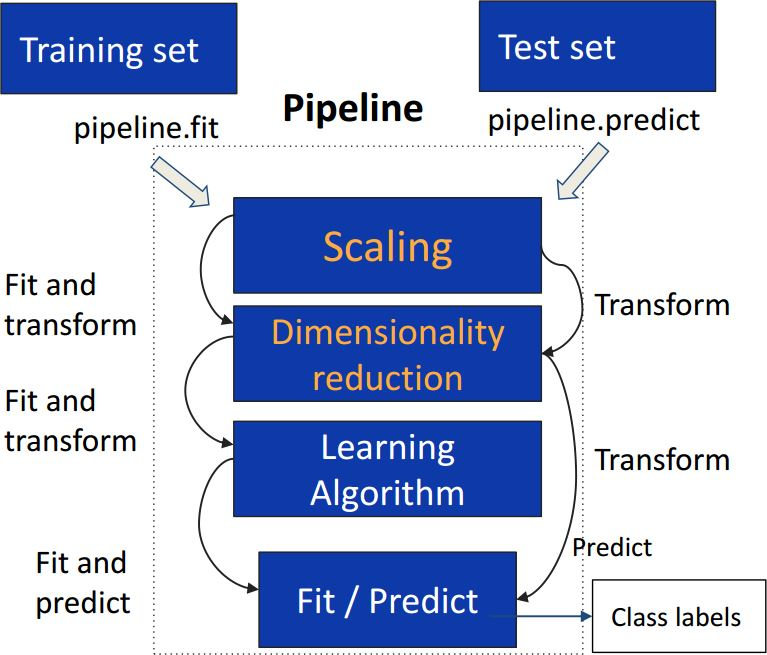
\includegraphics[width=3.0in]{pipelinebuilding1}
		\caption[Pipeline building]{Pipeline building.}
		\label{fig:pipelinebuilding1}
	\end{figure}

Note, a pipeline can be constructed purely for data transformation alone; it is not mandatory to have an estimator.


Specifying names for the different stages of a pipeline can lead to ambiguities. When there are multiple stages, each stage has to be uniquely named and we have to make sure there is consistency in the naming process such as usage of lower case letters only, each name should be unique, name should reflect the purpose of the stage etc. Manual naming is prone to errors.
Alternatively we can use \textcode{make\_pipeline()} function that will create the pipeline and automatically name each step as the lowercase of the name of the function called:

	\begin{code}[\codenumbering]{}
		\codeitemnonumber from sklearn.pipeline import make\_pipeline
		\codeitemnonumber pipe = make\_pipeline(MinMaxScaler(), (LogisticRegression()))
		\codeitemnonumber print("Pipeline steps:\ n{}". format(pipe.steps))
	\end{code}

The advantage of ``make\_pipeline'' is the consistency in the naming of each stage, we can have multiple stages in a pipeline performing the same transformations.  Each stage is guaranteed to have a unique, meaningful name.

	\section{Hyper Parameters and Tuning}

	\begin{numberedlist}
		\item Hyper parameters are like handles available to the modeler to control the behavior of the algorithm used for modeling
		\item Hyper parameters are supplied as arguments to the model algorithms while initializing them.  E.g., setting the criterion for decision tree building
		\begin{code}[\codenumbering]{}
			\codeitemnonumber dt\_model = DecisionTreeClassifier(criterion = 'entropy')
		\end{code}
		\item To get a list of hyper parameters for a given algorithm, call the function \textcode{get\_params()}.  E.g., to get support vector classifier hyper parameters
		\begin{code}[\codenumbering]{}
			\codeitemnonumber from sklearn.svm import SVC
			\codeitemnonumber svc = SVC()
			\codeitemnonumber svc.get\_params()
		\end{code}
		\item Hyperparameters are not learnt from the data as other model parameters are.  E.g., attribute coefficients in a linear model are learnt from data while cost of error is input as hyperparameter.
		\item Fine tuning the hyper parameters is done in a sequence of steps:
		\begin{numberedlist}
			\item Selecting the appropriate model type (regressor or classifier such as \textcode{sklearn.svm.SVC()})
			\item Identify the corresponding parameter space.
			\item Decide the method for searching or sampling parameter space.
			\item Decide the cross-validation scheme to ensure model will generalize
			\item Decide a score function to use to evaluate the model.
		\end{numberedlist}
		\item Two generic approaches to searching hyper parameter space include
		\begin{numberedlist}
			\item \textcode{GridSearchCV} which exhaustively considers all parameter combinations.
			\item \textcode{RandomizedSearchCV} can sample a given number of candidates from a parameter space with a specified distribution.
		\end{numberedlist}
		\item While tuning hyper parameters, the data should have been split into three parts (training, validation, and testing) to prevent data leak.
		\item The testing data should be separately transformed\footnote{ Any transformation where rows influence each other. E.g., using zscore. OneHotCode
transformation does not come into this category. It can be done before splitting the data.} using the same functions that were used to transform the rest of the data for model building and hyperparameter tuning.
	\end{numberedlist}

	\section{GridSearchCV}

	\begin{figure}[tbh]
		\centering
		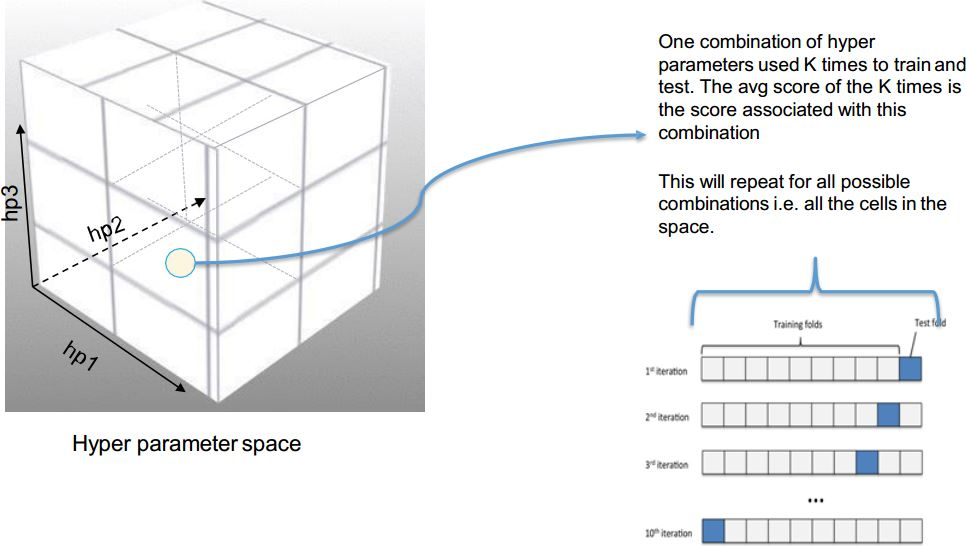
\includegraphics[width=\textwidth]{gridsearchcv}
		\caption[GridSearchCV]{GridSearchCV.}
		\label{fig:gridsearchcv}
	\end{figure}


	\section{\codefont RandomizedSearchCV}

	\begin{bulletedlist}
	\item Random search differs from grid search. Instead of providing a discrete set of values to explore on each hyperparameter (parameter grid), we provide a statistical distribution.
	\item Values for the different hyper parameters are picked up at random from this combine distribution.
	\item The motivation to use random search in place of grid search is that for many cases, hyperparameters are not equally important.  From Bergstra 2012, a Gaussian process analysis of the function from hyper-parameters to validation set performance reveals that for most data sets only a few of the hyper-parameters really matter, but that different hyper-parameters
are important on different data sets. This phenomenon makes grid search a poor choice for configuring algorithms for new data sets.
	\item In contrast to GridSearchCV, not all combinations are evaluated.  A fixed number of parameter settings is sampled from the specified distributions.
	\item The number of parameter settings that are tried is given by \textcode{n\_iter}.
	\item If all parameters are presented as a list, sampling without replacement is performed. If at least one parameter is given as a distribution, sampling with replacement is used. It is highly recommended to use continuous distributions for continuous parameters.
	\item RandomSearchCV has higher chance of hitting the right combination than GridSearchCV.
	\end{bulletedlist}

	\begin{figure}[tbh]
		\centering
		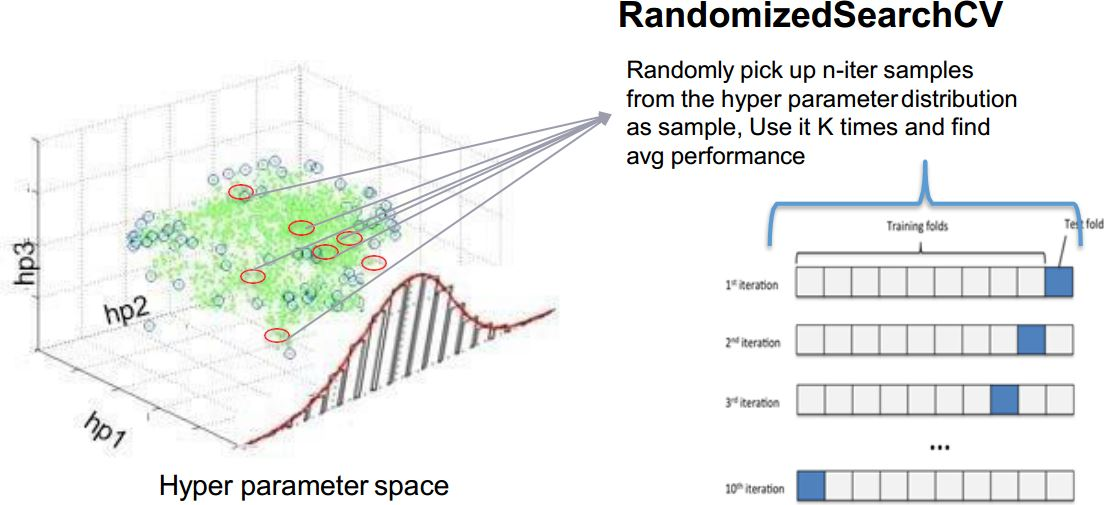
\includegraphics[width=\textwidth]{randomsearchcv }
		\caption[RandomSearchCV]{RandomSearchCV}
		\label{fig:randomsearchcv}
	\end{figure} 